\section{Introduction to Fourier series}

Every function $f(x)$ on domain $-L<x<L$ can be represented by a series of the form

\begin{equation*}
    A_0+\sum_{n=1}^{\infty}\left(A_n \cos \frac{n \pi x}{L}+B_n \sin \frac{n \pi x}{L}\right)
\end{equation*}

This is called the Fourier series. We will first discuss how to compute the coefficients $A_0, A_1, B_1$, $\dots$ in terms of $f(x)$, then we discuss several properties and variants of the Fourier series.

\subsection{Definition of Fourier series}

The Fourier series is an infinite sum of trigonometric functions defined as the following

\begin{definition}[Fourier series] Let $A_0, A_1, B_1, \ldots$ be constants. The series below is called a \underline{Fourier series}.
    \begin{equation}\label{eq.fourier_def}
        A_0+\sum_{n=1}^{\infty}\left(A_n \cos \frac{n \pi x}{L}+B_n \sin \frac{n \pi x}{L}\right)
    \end{equation}
\end{definition}

It turns out that every function $f(x)$ can be written into an infinite sum of trigonometric functions. As suggested by the following theorem,

\begin{theorem}[]
Every function $f(x)$ on domain $-L<x<L$ can be represented by a Fourier series. In other word, for any $f(x)$ on domain $-L<x<L$, there exists coefficients $A_0, A_1, B_1, \dots$ such that 
\begin{equation}\label{eq.fourier}
    f(x)=A_0+\sum_{n=1}^{\infty}\left(A_n \cos \frac{n \pi x}{L}+B_n \sin \frac{n \pi x}{L}\right) .
\end{equation}
\end{theorem}


\subsection{Fourier series and orthogonality}

\subsubsection{Orthogonality of trigonometric function}

We want to compute the coefficients $A_0, A_1, B_1$, $\dots$ in terms of $f(x)$. The following observation may be helpful.

\textbf{Question.} Given several orthogonal vector $e_1, e_2, \dots, e_n$, assume that we have a decomposition 
\begin{equation}\label{eq.vector_expansion}
    v = v_1e_1+v_2e_2+\cdots+v_ne_n
\end{equation}
How do we compute the coefficients $v_1, v_2, \dots, v_n$ in terms of $v$?

\textbf{Answer.} Assume that we want to solve the coefficient $v_j$, then we take inner product of \eqref{eq.vector_expansion} with $e_j$. If we do this, by orthogonality $\langle e_i, e_j\rangle = 0$ (if $i\ne j$) and $\langle e_j, e_j\rangle = |e_j|^2$, then we get
\begin{equation}\label{eq.vector_take_inner}
    \begin{split}
        \langle v, e_j\rangle =& \langle v_1e_1+v_2e_2+\cdots+v_ne_n, e_j\rangle 
        \\
        =& v_j  |e_j|^2.
    \end{split}
\end{equation}
Therefore, we solve the coefficient $v_j = \frac{\langle v, e_j\rangle}{|e_j|^2}$.

The following notation is useful.

\begin{definition}[Kronecker delta]
The \underline{Kronecker delta} $\delta_{m n}$ is defined as
\begin{equation}\label{eq.Kronecker_delta}
    \delta_{m n}= 
    \left\{
    \begin{aligned}
        &1, \quad && m=n 
        \\ 
        &0, \quad && m \neq n 
    \end{aligned}
    \right.
\end{equation}
Using this notation orthogonality of $e_1, e_2, \dots, e_n$ is equivalent to $\langle e_m, e_n\rangle = |e_m|^2\delta_{m n}$.
\end{definition}

The following theorem implies that sine and cosine functions are similar to orthogonal vectors.

\begin{theorem}[Orthogonality of trigonometric functions] Let $n, m \ge 0$ be integers. We assume $L>$ 0. The following orthogonality relations hold.
    \begin{equation}\label{eq.orthogonality}
        \begin{aligned}
            & \int_{-L}^L \cos \frac{n \pi x}{L} \cos \frac{m \pi x}{L} d x=\left\{
                \begin{aligned}
                &2 L \quad && (n=m=0), 
                \\
                &L \delta_{n m} \quad && (\text{otherwise}),
                \end{aligned}\right. 
            \\
            & \int_{-L}^L \sin \frac{n \pi x}{L} \sin \frac{m \pi x}{L} d x=\left\{
                \begin{aligned}
                &0 \quad &&  (n=m=0), 
                \\
                &L \delta_{n m} \quad &&  (\text {otherwise}),
                \end{aligned}\right. 
            \\
            & \int_{-L}^L \sin \frac{n \pi x}{L} \cos \frac{m \pi x}{L} d x=0 \quad(\text {all } n, m) .
            \end{aligned}
    \end{equation}
\end{theorem}
\begin{proof}
We only prove the orthogonality for the first equation which only involves cosine. The proof of other equations is left as homework. 

Let us first start with the following observation.

\textit{Claim.} If $n\neq 0$, then we have
\begin{equation}\label{eq.proof_orth_cos_int}
    \int_{-L}^L \cos \frac{n \pi x}{L} dx = 0
\end{equation}

This claim is true because
\begin{equation}\label{eq.proof_orth_cos_int_1}
    \begin{split}
        \int_{-L}^L \cos \frac{n \pi x}{L} dx =& \left[\frac{L}{n\pi}\sin \frac{n \pi x}{L}\right]^{L}_{-L} 
        \\
        =& \frac{L}{n\pi} (\sin n\pi - \sin (- n\pi) ) = 0
    \end{split}
\end{equation}

Now we start the proof of \eqref{eq.orthogonality} for cosine.

\textbf{Case 1.} ($n=m=0$) In this case, we have
$$
\int_{-L}^L \cos \frac{n \pi x}{L} \cos \frac{m \pi x}{L} d x=\int_{-L}^L 1 \cdot 1 d x=2 L
$$

\textbf{Case 2.} (At least one of $n, m$ is nonzero). We have
$$
\int_{-L}^L \cos \frac{n \pi x}{L} \cos \frac{m \pi x}{L} d x=\frac{1}{2} \int_{-L}^L\left(\cos \frac{(n-m) \pi x}{L}+\cos \frac{(n+m) \pi x}{L}\right) d x
$$

Since at least one of $n, m$ is nonzero, $n+m > 0$. The integral over $\cos \frac{(n+m) \pi x}{L}$ is $0$ by \eqref{eq.proof_orth_cos_int}.

Therefore,
$$
\int_{-L}^L \cos \frac{n \pi x}{L} \cos \frac{m \pi x}{L} d x=\frac{1}{2} \int_{-L}^L\cos \frac{(n-m) \pi x}{L} d x
$$

\textbf{Case 2.1.} ($n \neq m$) In this case, $\frac{1}{2} \int_{-L}^L\cos \frac{(n-m) \pi x}{L} d x = 0$ by \eqref{eq.proof_orth_cos_int}. Therefore, we get 
$$
\int_{-L}^L \cos \frac{n \pi x}{L} \cos \frac{m \pi x}{L} d x = 0 =\delta_{m n}.
$$


\textbf{Case 2.2.} ($n = m$), then
$$
\int_{-L}^L \cos \frac{n \pi x}{L} \cos \frac{m \pi x}{L} d x =\frac{1}{2} \int_{-L}^L\cos \frac{(n-m) \pi x}{L} d x =\frac{1}{2} \int_{-L}^L \cos \frac{0 \cdot \pi x}{L} d x=L .
$$

Thus the orthogonality relations for $\int_{-L}^L \cos \frac{n \pi x}{L} \cos \frac{m \pi x}{L} d x$ is proved. The orthogonality relations for $\int_{-L}^L \sin \frac{n \pi x}{L} \sin \frac{m \pi x}{L} d x$ and $\int_{-L}^L \sin \frac{n \pi x}{L} \cos \frac{m \pi x}{L} d x$ are similarly proved and left as homework.
\end{proof}



\subsubsection{Formula of Fourier coefficients}

\quad\, We can use the orthogonality relations \eqref{eq.orthogonality} to compute $A_0, A_1, B_1$, $\dots$

To determine $A_0$ in \eqref{eq.fourier}, we multiply $\cos \frac{0 \cdot \pi x}{L}=1$ on both sides and integrate with respect to $x$:
$$
\int_{-L}^L f(x) d x=\int_{-L}^L A_0 d x+\sum_{n=1}^{\infty} \int_{-L}^L\left(A_n \cos \frac{n \pi x}{L}+B_n \sin \frac{n \pi x}{L}\right) d x=\int_{-L}^L A_0 d x=2 A_0.
$$
where we use the fact that $\int_{-L}^L \cos \frac{n \pi x}{L} dx = \int_{-L}^L \sin \frac{n \pi x}{L} dx = 0$. This is just the first equation in \eqref{eq.orthogonality} with $m = 0$. 

Therefore, we get an expression of $A_0$,
$$
A_0=\frac{1}{2 L} \int_{-L}^L f(x) d x.
$$

To determine $A_m$ $(m=1,2, \ldots)$ in \eqref{eq.fourier}, we multiply $\cos \frac{m \pi x}{L}$ on both sides and integrate with respect to $x$:
$$
\begin{aligned}
\int_{-L}^L f(x) \cos \frac{m \pi x}{L} d x & =\int_{-L}^L A_0 \cos \frac{m \pi x}{L} d x+\sum_{n=1}^{\infty} \int_{-L}^L\left(A_n \cos \frac{n \pi x}{L}+B_n \sin \frac{n \pi x}{L}\right) \cos \frac{m \pi x}{L} d x \\
& =\sum_{n=1}^{\infty} A_n \int_{-L}^L \cos \frac{n \pi x}{L} \cos \frac{m \pi x}{L} d x=\sum_{n=1}^{\infty} A_n L \delta_{n m}=L A_m .
\end{aligned}
$$

Therefore, we get an expression of $A_m$,
$$
A_m = \int_{-L}^L f(x) \cos \frac{m \pi x}{L} d x.
$$

Similarly we can determine $B_m$ $(m=1,2, \ldots)$ in \eqref{eq.fourier} by multiplying $\sin \frac{m \pi x}{L}$ on both sides and integrate with respect to $x$:
$$
\begin{aligned}
\int_{-L}^L f(x) \sin \frac{m \pi x}{L} d x & =\int_{-L}^L A_0 \sin \frac{m \pi x}{L} d x+\sum_{n=1}^{\infty} \int_{-L}^L\left(A_n \cos \frac{n \pi x}{L}+B_n \sin \frac{n \pi x}{L}\right) \sin \frac{m \pi x}{L} d x \\
& =\sum_{n=1}^{\infty} B_n \int_{-L}^L \sin \frac{n \pi x}{L} \sin \frac{m \pi x}{L} d x=\sum_{n=1}^{\infty} B_n L \delta_{n m}=L B_m .
\end{aligned}
$$

Therefore, we get an expression of $B_m$,
$$
B_m = \int_{-L}^L f(x) \sin \frac{m \pi x}{L} d x.
$$

In summary, we have the following theorem.

\begin{theorem}[]
The Fourier coefficients in $A_0, A_1, B_1$, $\dots$ are given by
\begin{equation}\label{eq.fourier_coefficient}
    \begin{aligned}
        \,&A_0=\frac{1}{2 L} \int_{-L}^L f(x) d x, 
        \\
        &A_n=\frac{1}{L} \int_{-L}^L f(x) \cos \frac{n \pi x}{L} d x, 
        \\
        &B_n=\frac{1}{L} \int_{-L}^L f(x) \sin \frac{n \pi x}{L} d x.
    \end{aligned}
\end{equation}
\end{theorem}

\begin{example}[]\label{ex.x_fourier}
Let us calculate the Fourier series of $f(x)=x,-L<x<L$. 
\end{example}
\begin{proof}[Solution]
    We have
    $$
    \begin{aligned}
    & A_0=\frac{1}{2 L} \int_{-L}^L x d x=0, 
    \\
    & A_n=\frac{1}{L} \int_{-L}^L x \cos \frac{n \pi x}{L} d x=0 \quad (x \cos \frac{n \pi x}{L} \textit{ is an odd function}), 
    \\
    & B_n=\frac{1}{L} \int_{-L}^L x \sin \frac{n \pi x}{L} d x=\frac{1}{L}\left[-\left.\frac{L}{n \pi} x \cos \frac{n \pi x}{L}\right|_{-L} ^L+\frac{L}{n \pi} \int_{-L}^L \cos \frac{n \pi x}{L} d x\right]=\frac{2 L}{n \pi}(-1)^{n+1} .
    \end{aligned}
    $$
    
    Therefore we obtain
    \begin{equation}\label{eq.fourier_x}
        x=\sum_{n=1}^{\infty} \frac{2 L}{n \pi}(-1)^{n+1} \sin \frac{n \pi x}{L}, \quad-L<x<L .
    \end{equation}
    
\end{proof}

We have two observations from the above example

\begin{proposition}[]\label{prop.odd_even_sin_cos}
    An odd or even function only has $\cos$ or  $\sin$ term in its Fourier series.
\end{proposition}
\begin{proof}
    We only consider the even case. The odd case can be proved similarly. 
    
    Since $f(x)$ is even, we know that $\frac{1}{L} \int_{-L}^L f(x) \sin \frac{n \pi x}{L} d x$ is odd. By \eqref{eq.fourier_coefficient}, all the $B_n$ vanishes. Therefore, we only have the $\cos$ term in the Fourier series.
\end{proof}

\begin{proposition}[]
    Given a function $f(x)$ defined on $-L < x < L$, the Fourier series of $f(x)$ coincide with $f(x)$ only in the domain $-L < x < L$, unless $f(x)$ is a periodic function.
\end{proposition}
\begin{proof}
    We will not prove this proposition. Instead, we draw the graph of $y = x$ and its Fourier series

    The Fourier series coincides with $y = x$ only in the domain $-L < x < L$. But the Fourier series is a periodic function since it is a sum of several periodic functions $\cos/\sin$. Since $y = x$ is not a periodic function, the Fourier series cannot agree with it for all $x$.
    \begin{figure}[H]
        \begin{tikzpicture}
            \node at (0,0) {\scalebox{0.1}{      
                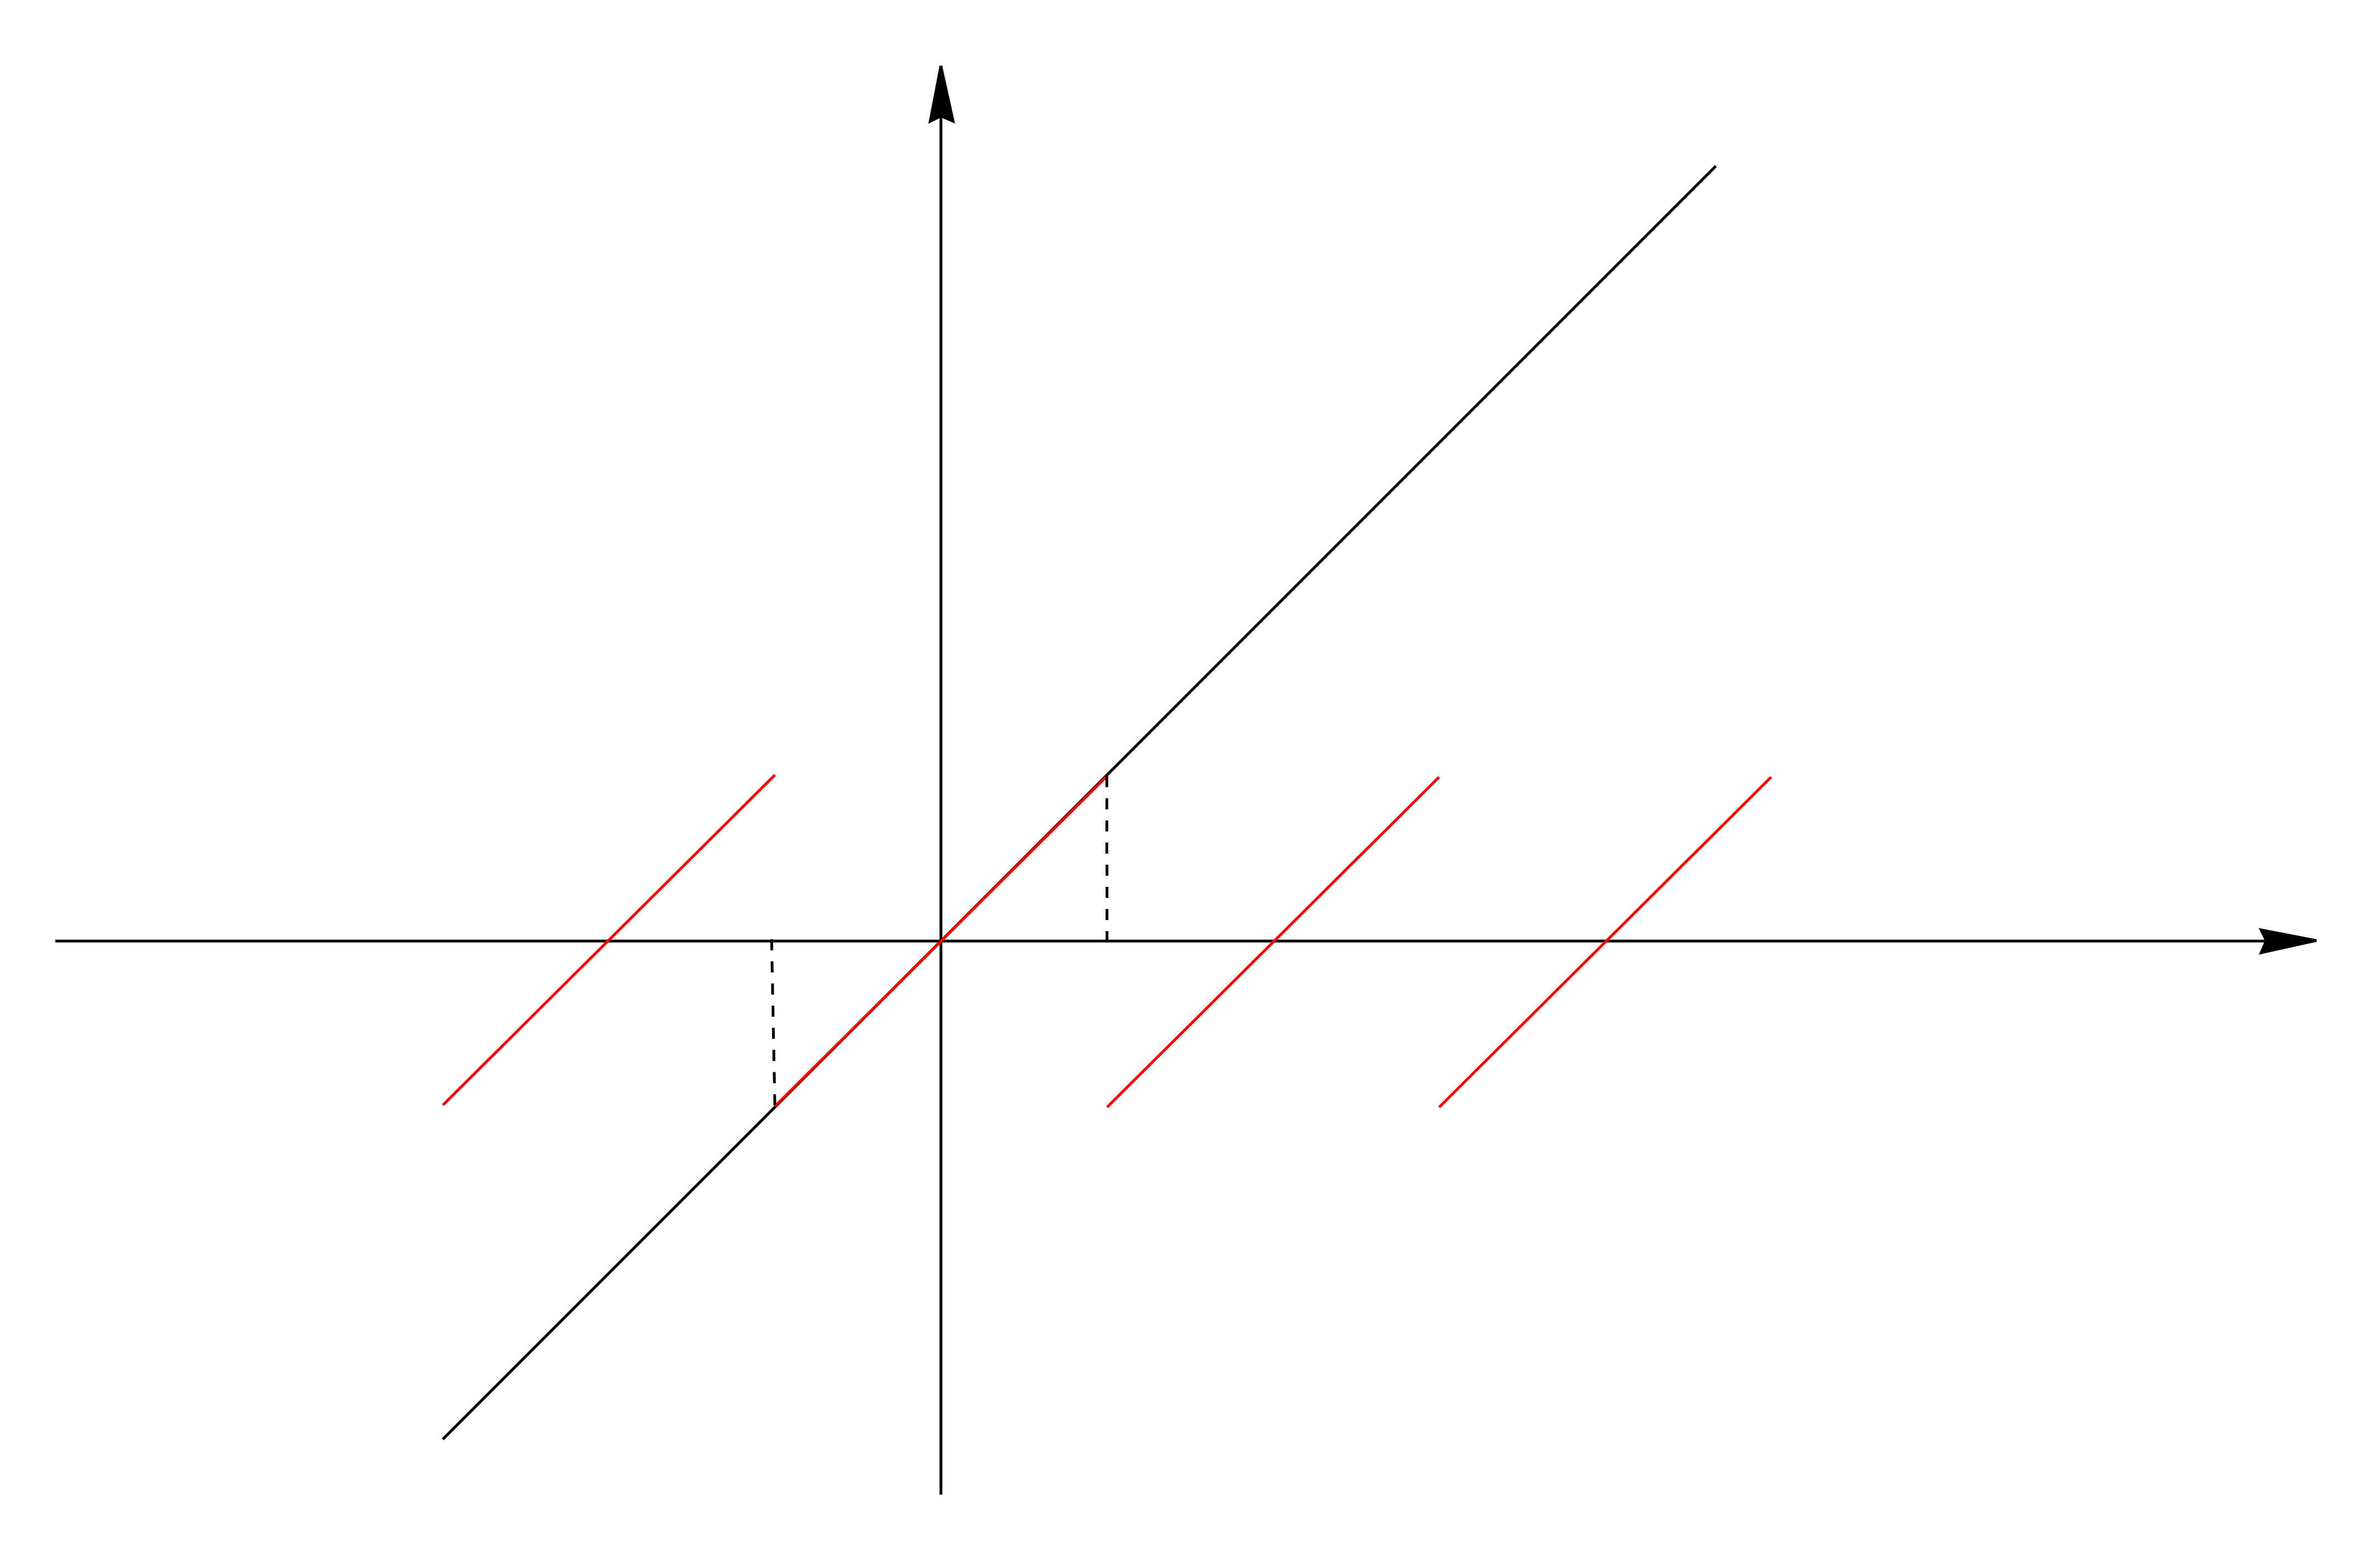
\includegraphics{pictures/fourier_x.png}
            }};
            \node at (2.5, 2) {$y = x$};
            \node at (5.25, -1.1) {$x$};
            \node at (-0.9, 3.2) {$y$};
            \node at (-0.4, -1.1) {$L$};
            \node at (-2, -1.1) {$-L$};
            \node at (4.1, -0.2) {\textit{Fourier series}};
        \end{tikzpicture}
        \centering 
        \caption{The graph of $y = x$ and its Fourier series.} 
        \label{fig.fourier_x} 
    \end{figure}
\end{proof}


\subsubsection{Solve the $A_n$ coefficients in \eqref{eq.match_boundary_1}}\label{sec.A_n_coef_sep} 

\quad\, Now we return to the separation of variable in section \ref{sec.match_boundary}, where we derived
\begin{equation}\label{eq.match_boundary_1_repeat}
    \varphi(x) =\sum_{n = 1}^{\infty} A_n \sinh n \pi \sin \frac{n \pi x}{L}.
\end{equation}

We want to solve $A_n$ from $\varphi(x)$.

As explained in section \ref{sec.fourier_cosine_sine}, on $0 < x < L$, we also have the following orthogonality of $\sin \frac{n \pi x}{L}$
\begin{equation}\label{eq.solve_A_n_1}
    \int_{0}^L \sin \frac{n \pi x}{L} \sin \frac{m \pi x}{L} d x= \frac{L}{2} \delta_{n m}, \qquad n,m\ge 1.
\end{equation}

Therefore, if we want to solve $A_m$, we can multiply \eqref{eq.match_boundary_1_repeat} by  $\sin \frac{n \pi x}{L}$ and then integrate over $x$
$$
\begin{aligned}
&\int_{0}^L \varphi(x) \sin \frac{m \pi x}{L} d x  = \sum_{n=1}^{\infty} \int_{0}^L A_n \sinh n \pi \sin \frac{n \pi x}{L} \sin \frac{m \pi x}{L} d x \\
=&\sum_{n=1}^{\infty}  A_n \sinh n \pi \int_{0}^L \sin \frac{n \pi x}{L} \sin \frac{m \pi x}{L} d x=\sum_{n=1}^{\infty}  A_n \sinh n \pi \frac{L}{2} \delta_{n m}= \frac{L}{2} A_m \sinh n \pi .
\end{aligned}
$$

From this, we can solve $A_m$ and get
\begin{equation}\label{eq.solve_A_n_2}
    A_n = \frac{2}{L\sinh n\pi}\int_{0}^{L}\varphi(x)\sin \frac{n \pi x}{L} dx
\end{equation}

This is exactly \eqref{eq.solve_A_n}.

\subsection{Complex form of Fourier series}

We have seen that every function defined on $-L < x < L$ can be rewritten as an infinite sum of $\cos \frac{n \pi x}{L}$ and $\sin \frac{n \pi x}{L}$. By Euler's formula $e^{ix} = \cos x + i\sin x$, we know that every trigonometric function is a linear combination of $e^{ix}$ and $e^{-ix}$
\begin{equation}\label{eq.cos_sin_to_e^ix}
    \cos x = \frac{e^{ix}+e^{-ix}}{2}, \qquad \sin x = \frac{e^{ix}-e^{-ix}}{2i}.
\end{equation}

Therefore, we have the following theorem.
\begin{theorem}[]
    In other word, for any $f(x)$ on domain $-L<x<L$, there exists coefficients $\dots, \alpha_{-1}, \alpha_0, \alpha_1, \alpha_2, \dots$ such that 
    \begin{equation}\label{eq.fourier_complex}
        f(x)=\sum_{n=-\infty}^{\infty} \alpha_n e^{i n \pi x / L},
    \end{equation}
    where $\alpha_n$ satisfies the following properties.
    \begin{enumerate}
        \item $\alpha_n$ is given by 
        \begin{equation}\label{eq.fourier_complex_coefficients}
            \alpha_n=\frac{1}{2 L} \int_{-L}^L f(x) e^{-i n \pi x / L} d x
        \end{equation}
        \item If $f(x)$ is a real value function, then $\alpha_n = \bar{\alpha}_{-n}$, where $\bar{\alpha}_{-n}$ is the complex conjugate of $\alpha_{-n}$.
    \end{enumerate}
\end{theorem}
\begin{proof}
Using Euler's formula \eqref{eq.cos_sin_to_e^ix}, we can rewrite the Fourier series of $f$ as follows.
$$
\begin{aligned}
    f(x)=&A_0+\sum_{n=1}^{\infty}\left(A_n \cos \frac{n \pi x}{L}+B_n \sin \frac{n \pi x}{L}\right)
    \\
    =& A_0+\sum_{n=1}^{\infty}\left(A_n \left(\frac{e^{i n \pi x / L} + e^{-i n \pi x / L}}{2}\right)+B_n \left(\frac{e^{i n \pi x / L} - e^{-i n \pi x / L}}{2i}\right)\right)
    \\
    =&A_0+\sum_{n=1}^{\infty}\left(\frac{A_n-i B_n}{2} e^{i n \pi x / L}+\frac{A_n+i B_n}{2} e^{-i n \pi x / L}\right) .
\end{aligned}
$$

If we define
\begin{equation}\label{eq.alpha_to_A_B}
    \alpha_0=A_0, \quad \alpha_n=\frac{A_n-i B_n}{2}, \quad \alpha_{-n}=\frac{A_n+i B_n}{2}, \quad(n>0)
\end{equation}
then we obtain
$$
f(x)=\alpha_0+\sum_{n=1}^{\infty}\left(\alpha_n e^{i n \pi x / L}+\alpha_{-n} e^{-i n \pi x / L}\right)=\sum_{n=-\infty}^{\infty} \alpha_n e^{i n \pi x / L} .
$$

If $f(x)$ is a real value function, then $A_n$ and $B_n$ are real numbers. From \eqref{eq.alpha_to_A_B}, we know that $\alpha_n = \bar{\alpha}_{-n}$.

The formula of $\alpha_n$ is also a corollary of \eqref{eq.alpha_to_A_B}. When $n > 0$,
$$
\begin{aligned}
    \alpha_n =& \frac{A_n-i B_n}{2} = \frac{1}{2L} \int_{-L}^L f(x) \cos \frac{n \pi x}{L} d x -  \frac{i}{2L} \int_{-L}^L f(x) \sin \frac{n \pi x}{L} d x 
    \\
    =& \frac{1}{2 L} \int_{-L}^L f(x) e^{-i n \pi x / L} d x
\end{aligned}
$$

When $n = -m < 0$,
$$
\begin{aligned}
    \alpha_n = \alpha_{-m} =& \frac{A_{m}+i B_{m}}{2} = \frac{1}{2L} \int_{-L}^L f(x) \cos \frac{m \pi x}{L} d x + \frac{i}{2L} \int_{-L}^L f(x) \sin \frac{m \pi x}{L} d x 
    \\
    =& \frac{1}{2 L} \int_{-L}^L f(x) e^{i m \pi x / L} d x = \frac{1}{2 L} \int_{-L}^L f(x) e^{- i n \pi x / L} d x
\end{aligned}
$$

When $n = 0$,
$$
\alpha_0 = A_0 = \frac{1}{2L} \int_{-L}^L f(x) d x = \frac{1}{2 L} \int_{-L}^L f(x) e^{- i 0 \pi x / L} d x
$$
Therefore, we have completed the proof.
\end{proof}

$e^{i n \pi x / L}$ also have orthogonality relations.

\begin{theorem}[Orthogonality relations of complex Fourier series]
$$
\int_{-L}^L e^{i n \pi x / L} e^{-i m \pi x / L} d x=\int_{-L}^L e^{i(n-m) \pi x / L} d x=2 L \delta_{m n} .
$$
\end{theorem}
\begin{proof}
If $n = m$, 
$$
\int_{-L}^L e^{i(n-m) \pi x / L} d x = \int_{-L}^L 1 d x = 2L = 2L\delta_{m n}.
$$

If $n \neq m$, 
$$
\int_{-L}^L e^{i(n-m) \pi x / L} d x = \frac{L}{i\pi(n-m)}\left[e^{i(n-m) \pi x / L}\right]^{L}_{-L} = 0 = 2L\delta_{m n}.
$$

We have completed the proof.
\end{proof}

The formula of $\alpha_n$ can also be computed using orthogonality.

Assume that we want to compute $\alpha_m$ in 
$$
f(x)=\sum_{n=-\infty}^{\infty} \alpha_n e^{i n \pi x / L}.
$$

Multiply both side by $e^{-i m \pi x / L}$ and then we get
$$
\int_{-L}^L f(x) e^{-i m \pi x / L} d x=\sum_{n=-\infty}^{\infty} \alpha_n \int_{-L}^Le^{i n \pi x / L} e^{- i m \pi x / L} dx \sum_{n=-\infty}^{\infty} \alpha_n 2L \delta_{m n} = 2L\alpha_m.
$$

Solve $\alpha_m$, then we prove \eqref{eq.fourier_complex_coefficients} again.

\subsection{Fourier cosine and sine series}\label{sec.fourier_cosine_sine}

A function defined on $-L<x<L$ can be rewritten as an infinite sum of $\cos \frac{n \pi x}{L}$ and $\sin \frac{n \pi x}{L}$. Notice that $-L<x<L$ is the period of $\cos \frac{n \pi x}{L}$ and $\sin \frac{n \pi x}{L}$. If a function $f(x)$ is defined in the interval $0 < x < L$, which represents half of its period, then it is possible to express $f(x)$ exclusively as a series of cosine terms, $\cos \frac{n \pi x}{L}$, or alternatively, only as a series of sine terms, $\sin \frac{n \pi x}{L}$. This is the Fourier cosine/sine series.

The idea is that, given a function $f(x)$ defined on $0 < x < L$, we can extend this function as an even/odd function on $-L < x < L$. Then we compute the Fourier series of the extended function. The Fourier series only contains $\cos \frac{n \pi x}{L}$ or $\sin \frac{n \pi x}{L}$ terms by Proposition \ref{prop.odd_even_sin_cos}.

\subsubsection{Fourier cosine series}


We define the even extension $f_E(x)$ of $f(x)$ as
\begin{equation}\label{eq.even_extension}
    f_E(x)=\left\{\begin{aligned}
        &f(x), && 0<x<L 
        \\
        &\,0, && x=0, 
        \\
        &f(-x), && -L<x<0 .
        \end{aligned}\right.
\end{equation}

We note that $f_E(x)$ is even. Indeed the value $f_E(0)$ is arbitrary and not necessarily zero. The Fourier series is given by
$$
f_E(x)=A_0+\sum_{n=1}^{\infty} A_n \cos \frac{n \pi x}{L}, \quad-L<x<L,
$$
where
$$
\begin{aligned}
& A_0=\frac{1}{2 L} \int_{-L}^L f_E(x) d x=\frac{1}{L} \int_0^L f(x) d x, \\
& A_n=\frac{1}{2 L} \int_{-L}^L f_E(x) \cos \frac{n \pi x}{L} d x=\frac{2}{L} \int_0^L f(x) \cos \frac{n \pi x}{L} d x .
\end{aligned}
$$

On the interval $0<x<L$ we have
\begin{equation}\label{eq.fourier_cosine}
    f(x)=A_0+\sum_{n=1}^{\infty} A_n \cos \frac{n \pi x}{L}, \quad 0<x<L,
\end{equation}
where
\begin{equation}\label{eq.fourier_cosine_coefficient}
    A_0=\frac{1}{L} \int_0^L f(x) d x, \quad A_n=\frac{2}{L} \int_0^L f(x) \cos \frac{n \pi x}{L} d x .
\end{equation}


\begin{definition}[]
    The series \eqref{eq.fourier_cosine} is called the Fourier cosine series.
\end{definition}

For Fourier cosine series, we also have orthogonality relations and \eqref{eq.fourier_cosine_coefficient} can be computed from these orthogonality relations.

\begin{theorem}[Orthogonality relations of cosine Fourier series]
    \begin{equation}\label{eq.cosine_orthogonality}
        \int_{0}^L \cos \frac{n \pi x}{L} \cos \frac{m \pi x}{L} d x=\left\{
                \begin{aligned}
                &L \quad && (n=m=0), 
                \\
                &\frac{L}{2} \delta_{n m} \quad && (\text{otherwise}),
                \end{aligned}\right.
    \end{equation}
\end{theorem}

\begin{example}[]\label{ex.|x|_fourier}
    Let us compute the Fourier cosine series of $f(x)=x$, $0<x<L$.
\end{example}
\begin{proof}[Solution]
We can directly apply \eqref{eq.fourier_cosine_coefficient}. But let us try the even extension method.
    
We extend $f$ as
$$
f_E(x)=\left\{\begin{aligned}
&\,x, && \,0<x<L, \\
&\,0, && \,x=0, \\
&-x, && -L<x<0 .
\end{aligned}\right.
$$

Indeed $f_E(x)=|x|$.
$$
\begin{aligned}
A_0 & =\frac{1}{2 L} \int_{-L}^L f_E(x) d x=\frac{1}{L} \int_0^L x d x=\frac{L}{2}, \\
A_n & =\frac{1}{2 L} \int_{-L}^L f_E(x) \cos \frac{n \pi x}{L} d x=\frac{2}{L} \int_0^L x \cos \frac{n \pi x}{L} d x \\
& =\frac{2}{L}\left[\left.\frac{L}{n \pi} x \sin \frac{n \pi x}{L}\right|_0 ^L-\frac{L}{n \pi} \int_0^L \sin \frac{n \pi x}{L} d x\right]=\frac{2 L}{(n \pi)^2}\left((-1)^n-1\right) .
\end{aligned}
$$

Therefore,
$$
x=\frac{L}{2}+\frac{2 L}{\pi^2} \sum_{n=1}^{\infty} \frac{(-1)^n-1}{n^2} \cos \frac{n \pi x}{L}, \quad 0<x<L .
$$
\end{proof}


\subsubsection{Fourier sine series}

We define the odd extension $f_O(x)$ as
\begin{equation}\label{eq.odd_extension}
    f_O(x)=\left\{\begin{aligned}
        &f(x), && 0<x<L 
        \\
        &\,0, && x=0, 
        \\
        &-f(-x), && -L<x<0 .
        \end{aligned}\right.
\end{equation}

We note that $f_O(x)$ is odd. The Fourier series is given by
$$
f_O(x)=\sum_{n=1}^{\infty} B_n \sin \frac{n \pi x}{L}, \quad-L<x<L,
$$
where
$$
B_n=\frac{1}{L} \int_{-L}^L f_O(x) \sin \frac{n \pi x}{L} d x=\frac{2}{L} \int_0^L f(x) \sin \frac{n \pi x}{L} d x .
$$

On the interval $0<x<L$ we have
\begin{equation}\label{eq.fourier_sine}
    f(x)=\sum_{n=1}^{\infty} B_n \sin \frac{n \pi x}{L}, \quad 0<x<L,
\end{equation}
where
\begin{equation}\label{eq.fourier_sine_coefficient}
    B_n=\frac{2}{L} \int_0^L f(x) \sin \frac{n \pi x}{L} d x
\end{equation}

\begin{definition}[]
    The series \eqref{eq.fourier_sine} is called the Fourier cosine series.
\end{definition}

For Fourier sine series, we also have orthogonality relations and \eqref{eq.fourier_sine_coefficient} can be computed from these orthogonality relations.

\begin{theorem}[Orthogonality relations of sine Fourier series]
    \begin{equation}\label{eq.sine_orthogonality}
        \int_{0}^L \sin \frac{n \pi x}{L} \sin \frac{m \pi x}{L} d x=\left\{
                \begin{aligned}
                &0 \quad && (n=m=0), 
                \\
                &\frac{L}{2} \delta_{n m} \quad && (\text{otherwise}),
                \end{aligned}\right.
    \end{equation}
\end{theorem}

\begin{example}
    The Fourier sine series of $f(x)=x$, $0<x<L$, is obtained through the odd extension $f_O(x)$. The odd extension $f_O(x)$ is again $x$ and its Fourier series has been computed in \eqref{eq.fourier_x}.
\end{example}


\subsection{Convergence of Fourier series}

In this section, we study the convergence of Fourier series of piecewise continuous functions.

\begin{definition}[Left and right limits]
For a given $f(x)$, let us write
\begin{equation}\label{eq.left_right_limit}
    f(x+0)=\lim _{\varepsilon \rightarrow 0} f(x+\varepsilon), \quad f(x-0)=\lim _{\varepsilon \rightarrow 0} f(x-\varepsilon),
\end{equation}
where $\varepsilon>0$.
\end{definition}


\begin{definition}[Piecewise continuous]
    A function $f(x)$ defined on $a<x<b$, is said to be \underline{piecewise continuous} if there is a finite set of points $a=x_0<x_1<\cdots<x_p<x_{p+1}=b$ such that $f(x)$ is continuous at $x \neq x_i$ $(i=1, \ldots, p)$, $f(x_i+0)(i=0, \ldots, p)$ exists, and $f(x_i-0)$ $(i=1, \ldots, p+1)$ exists.
\end{definition}

\begin{definition}[Piecewise smooth]
    A function $f(x), a<x<b$, is said to be \underline{piecewise smooth} if $f(x)$ and all of its derivatives are piecewise continuous.
\end{definition}



\begin{example}[]
    The function $f(x)=|x|,-L<x<L$, is piecewise smooth. The function $f(x)=x^2 \sin (1 / x)$,$-L<x<L$, is piecewise continuous but is not piecewise smooth because $\lim _{\varepsilon \rightarrow 0} f^{\prime}(0 \pm \varepsilon)$ does not exist. The function $f(x)=1 /\left(x^2-L^2\right)$, $-L<x<L$, is not piecewise continuous because $f(-L+0)$ and $f(L-0)$ are not finite.
\end{example}

\begin{definition}[Convergence]\label{def.convergence}
Given a Fourier series $f(x) = A_0+\sum_{n=1}^{\infty}[A_n \cos (n \pi x / L)+B_n \sin (n \pi x / L)]$, we define
\begin{enumerate}
    \item \textbf{Partial sums.} The \underline{partial sum}, denoted by $f_N(x)$, is defined to be
    \begin{equation}\label{eq.partial_sum}
        f_N(x)=A_0+\sum_{n=1}^N\left[A_n \cos (n \pi x / L)+B_n \sin (n \pi x / L)\right] .
    \end{equation}
    \item \textbf{Convergence at $x$.} We say the Fourier is \underline{convergent at $x$} if 
    \begin{equation}\label{eq.convergence_at_x}
        \lim_{N\rightarrow\infty}f_N(x) = f(x).
    \end{equation}
    \item \textbf{Uniformly convergence.} We say the Fourier is \underline{uniformly convergent} if 
    \begin{equation}\label{eq.convergence_uniformly}
        \lim_{N\rightarrow\infty} \max_{x\in [-L,L]}|f_N(x) - f(x)| = 0.
    \end{equation}
    This means that the convergence is equally well for all $x$.
\end{enumerate}

\end{definition}

\begin{theorem}[Convergence theorem]\label{th.convergence}
Let $f(x)$, $-L<x<L$, be piecewise smooth. Then the Fourier series of $f$ converges for all $x$ to the value $\frac{1}{2}[\bar{f}(x+0)+\bar{f}(x-0)]$, where $\bar{f}$ is the $2 L$-periodic function which equals to $f$ on $-L<x<L$.

If $f(x)$ is continuous on $[-L, L]$ and $f(-L)=f(L)$ in addition to the conditions assumed in the above theorem, then the Fourier series uniformly converges.
\end{theorem}

\begin{example}[] Here are two examples of convergence.

    \begin{enumerate}
        \item The Fourier series of $f(x)=|x|$, $-L<x<L$, (see Example \ref{ex.|x|_fourier}) uniformly converges. 
        
        \item The Fourier series of $f(x)=x$, $-L<x<L$ does not uniformly converge but converges at any point to $f(x)$ except for $x = -L$, $L$. 
    \end{enumerate}

    As in the following picture, the Fourier series of $f(x)=x$, $-L<x<L$ has a very bad convergence near $x = -L$, $L$, but the series of $f(x)=|x|$ has much better convergence.

    \textbf{TODO: add a picture}
\end{example}

\subsection{Parseval's Theorem and Mean Square Error}

\subsubsection{The Parseval's Theorem for Fourier series}

For orthogonal vectors $e_1,\dots, e_{n}$, $e_i\perp e_j$, their linear combination $v = v_1 e_1+\cdots+v_n e_n$ satisfies the Pythagorean theorem
\begin{equation}\label{eq.Pythagorean}
    |v|^2 = |v_1 e_1+\cdots+v_n e_n|^2 = |v_1 e_1|^2+\cdots+|v_n e_n|^2
\end{equation}

The proof of \eqref{eq.Pythagorean} is given by 
\begin{equation*}
    |v|^2 = \left\langle\sum_{j = 1}^{n}v_j e_j, \sum_{k = 1}^{n}v_k e_k\right\rangle = \sum_{j = 1}^{n}\sum_{k = 1}^{n}v_jv_k\underbrace{\langle e_j, e_k\rangle}_{= 0\textit{ if }j\neq k} = \sum_{j = 1}^{n}v_j^2 |e_j|^2
\end{equation*}

For the Fourier series, the following theorem claims that a similar identity is true.

\begin{theorem}[Parseval's theorem]\label{th.Parseval}
    Let $f(x)$ defined on $-L<x<L$ be a piecewise smooth function with Fourier series 
    \begin{equation}\label{eq.Parseval_assumption}
        f(x) = A_0+\sum_{n=1}^{\infty}[A_n \cos (n \pi x / L)+B_n \sin (n \pi x / L)]
    \end{equation}
    Then, the mean square $\frac{1}{2 L} \int_{-L}^L f(x)^2 d x$ of $f(x)$ satisfies the following identity
    \begin{equation}\label{eq.Parseval_fourier}
        \frac{1}{2 L} \int_{-L}^L f(x)^2 d x=A_0^2+\frac{1}{2} \sum_{n=1}^{\infty}\left(A_n^2+B_n^2\right)
    \end{equation}
\end{theorem}
\begin{proof}
    Since $\cos (0 \pi x / L) = 1$ and $\sin (0 \pi x / L) = 0$, we know that \eqref{eq.Parseval_assumption} is equivalent to 
    \begin{equation}\label{eq.proof_Parseval_1}
        \begin{split}
            f(x) =& \sum_{n=0}^{\infty}[A_n \cos (n \pi x / L)+B_n \sin (n \pi x / L)]
            \\
            =&\sum_{n=0}^{\infty}(A_n \cos_n +B_n \sin_n)
        \end{split}
    \end{equation}
    where we introduce the notation
    \begin{equation}\label{eq.proof_Parseval_2}
        \cos_n = \cos (n \pi x / L),\quad \sin_n = \sin (n \pi x / L)
    \end{equation}

    Similar to \eqref{eq.Pythagorean} and its proof, we have 
    \begin{equation}\label{eq.proof_Parseval_3}
        \begin{split}
            \frac{1}{2 L} \int_{-L}^L f(x)^2 d x 
            =& \frac{1}{2 L} \int_{-L}^L \sum_{n=0}^{\infty}[A_n \cos_n+B_n \sin_n] \sum_{m=0}^{\infty}[A_m \cos_m+B_m \sin_m] d x
            \\
            =&\frac{1}{2 L} \int_{-L}^L \sum_{n,m=0}^{\infty}(A_nA_m \underbrace{\cos_n\cos_m}_{= 0\textit{ if }n\neq m} + A_nB_m\underbrace{\cos_n\sin_m}_{=0} 
            \\
            &\qquad\qquad\quad+ B_nA_m\underbrace{\sin_n\cos_m}_{=0} + B_nB_m\underbrace{\sin_n\sin_m}_{= 0\textit{ if }n\neq m}) d x
            \\
            =&A_0^2+\frac{1}{2} \sum_{n=1}^{\infty}\left(A_n^2+B_n^2\right)
        \end{split}
    \end{equation}
    where in the last line, we applied the orthogonality of trigonometric functions \eqref{eq.orthogonality}.
\end{proof}

\subsubsection{The mean square error}

\begin{definition}[Mean square error]
We define the \underline{mean square error} $\sigma_N^2$ as
\begin{equation}\label{eq.mean_square_error}
    \sigma_N^2=\frac{1}{2 L} \int_{-L}^L[f(x)-f_N(x)]^2 d x
\end{equation}
where $f_N(x)$ is the partial sum
\begin{equation}
    f_N(x)=A_0+\sum_{n=1}^N\left[A_n \cos (n \pi x / L)+B_n \sin (n \pi x / L)\right] .
\end{equation}
\end{definition}

By Parseval's theorem, we obtain the following expression of the mean square error.

\begin{proposition}[] Given a partial summation whose mean square error is defined by \eqref{eq.mean_square_error}, then we have
    \begin{equation}\label{eq.mean_square_error_Parseval}
        \sigma_N^2=\frac{1}{2} \sum_{n=N+1}^{\infty}\left(A_n^2+B_n^2\right)
    \end{equation}
\end{proposition}
\begin{proof}
    This is an easy corollary of the Parseval's identity \eqref{eq.Parseval_fourier}, if we notice that
    $$
    f(x)-f_N(x) = \sum_{n=N+1}^\infty\left[A_n \cos (n \pi x / L)+B_n \sin (n \pi x / L)\right]
    $$ 
Therefore, we finished the proof.
\end{proof}

\begin{example}[]
Let us find $\sigma_N^2$ for $f(x)=x$, $-L<x<L$. 
\end{example}
\begin{proof}[Solution]
From Example \ref{ex.x_fourier}, we have $A_0=A_n=0$ and
\begin{equation}\label{eq.x_fourier_repeat}
    f_N(x)=\sum_{n=1}^N B_n \sin \frac{n \pi x}{L}, \quad B_n=\frac{2 L}{n \pi}(-1)^{n+1} .
\end{equation}

By \eqref{eq.mean_square_error_Parseval}, we obtain
$$
\sigma_N^2=\frac{1}{2} \sum_{n=N+1}^{\infty}\left(\frac{2 L}{n \pi}(-1)^{n+1}\right)^2=\frac{2 L^2}{\pi^2} \sum_{n=N+1}^{\infty} \frac{1}{n^2} .
$$

By Theorem \ref{th.int_test}, we get
$$
\int_{N+1}^{\infty} \frac{1}{x^2} d x \leq \sum_{n=N+1}^{\infty} \frac{1}{n^2} \leq \int_{N+1}^{\infty} \frac{1}{(x-1)^2} d x=\int_N^{\infty} \frac{1}{x^2} d x .
$$

We have
$$
\int_{N+1}^{\infty} \frac{1}{x^2} d x=\frac{1}{N+1} \ge \frac{1}{N} - \frac{1}{N^2}, \quad \int_N^{\infty} \frac{1}{x^2} d x=\frac{1}{N} .
$$

Let us introduce the symbol $O$ (this is called ``big O'') to express the order. For some $f_N$, $f_N=O\left(N^{-1}\right)$ as $N \rightarrow \infty$ means that there exist a constant $C>0$ such that $\left|f_N\right| \leq C N^{-1}$. Therefore we obtain
\begin{equation}\label{eq.x_fourier_mse_converge}
    \sigma_N^2=\frac{2 L^2}{\pi^2} \frac{1}{N}\left[1+O\left(\frac{1}{N}\right)\right]=O\left(N^{-1}\right), \quad N \rightarrow \infty .
\end{equation}

We note that $\sigma_N^2$ goes to zero as $N \rightarrow \infty$ although we know that the sum in \eqref{eq.x_fourier_repeat} does not converge uniformly. This happened because we considered the mean square and took the integral. \textbf{TODO: add a picture for convergence}
\end{proof}

\begin{theorem}[Integral test]\label{th.int_test}
    Given a monotonic and positive function $f(x)$, we have 
    \begin{equation}\label{eq.integral_test}
        \int^{\infty}_{N+1} f(x) dx \le \sum_{n = N+1}^{\infty} f(n)\le \int^{\infty}_{N} f(x) dx
    \end{equation}    
\end{theorem}
\begin{proof}
    \textbf{TODO: compare the area below the graph of $y = f(x)$}

    \textbf{TODO: add a picture}
\end{proof}

\begin{example}[]
Let us find $\sigma_{2 N}^2$ for $f(x)=|x|,-L<x<L$.
\end{example}
\begin{proof}[Solution]
From Example \ref{ex.|x|_fourier} we know that $B_n=0$, $A_{2 m}=0$ $(m=1,2, \ldots)$, and
$$
f_{2 N}(x)=A_0+\sum_{m=1}^N A_{2 m-1} \cos \frac{(2 m-1) \pi x}{L}, \quad A_0=\frac{L}{2}, \quad A_{2 m-1}=-\frac{4 L}{\pi^2(2 m-1)^2} .
$$

This is also the Fourier cosine series of $x$, $0<x<L$, in Example \ref{ex.|x|_fourier}. Hence we obtain
$$
\sigma_{2 N}^2=\frac{1}{2} \sum_{n=2 N+1}^{\infty} A_n^2=\frac{1}{2} \sum_{m=N+1}^{\infty} A_{2 m-1}^2=\frac{8 L^2}{\pi^4} \sum_{m=N+1}^{\infty} \frac{1}{(2 m-1)^4} .
$$

Note that by Theorem \ref{th.int_test}
$$
\int_{N+1}^{\infty} \frac{1}{(2 x-3)^4} d x \leq \sum_{m=N+1}^{\infty} \frac{1}{(2 m-1)^4} \leq \int_{N+1}^{\infty} \frac{1}{(2 x-1)^4} d x,
$$
and by Taylor expansion $\frac{1}{(1+x)^3} = 1 - 3x + 6x^2 + \cdots$, $\textit{LHS} = \frac{1}{8N^3}\frac{1}{(1+1/2N)^3}=\frac{1}{6(2 N+1)^3}=\frac{1}{48 N^3}+O\left(N^{-4}\right)$ and $\textit{RHS}=\frac{1}{6(2 N-1)^3}=\frac{1}{48 N^3}+O\left(N^{-4}\right)$.
Therefore we obtain
\begin{equation}\label{eq.|x|_fourier_mse_converge}
    \sigma_{2 N}^2=\frac{L^2}{6 \pi^4 N^3}+O\left(N^{-4}\right)=O\left(N^{-3}\right), \quad N \rightarrow \infty .
\end{equation}

Thus the Fourier series of $x$ converges as $O(1 / N)$ and the Fourier series of $|x|$ converges as $O\left(1 / N^3\right)$. Equations \eqref{eq.x_fourier_mse_converge} and \eqref{eq.|x|_fourier_mse_converge} explain the difference between figure \ref{fig.}.
\end{proof}

\subsubsection{Parseval's theorem for complex, cosine and sine Fourier series}


\begin{theorem}[Parseval's theorem for complex Fourier series]
    Let $f(x)$ defined on $-L<x<L$ be a piecewise smooth function with Fourier series 
    \begin{equation}\label{eq.Parseval_complex_assumption}
        f(x)=\sum_{n=-\infty}^{\infty} \alpha_n e^{i n \pi x / L}
    \end{equation}
    Then, the mean square $\frac{1}{2 L} \int_{-L}^L f(x)^2 d x$ of $f(x)$ satisfies the following identity
    \begin{equation}\label{eq.Parseval_complex}
        \frac{1}{2 L} \int_{-L}^L |f(x)|^2 d x=\sum_{n=-\infty}^{\infty}\left|\alpha_n\right|^2 .
    \end{equation}
\end{theorem}
\begin{proof}
\textit{Method 1.} We have 
\begin{equation}\label{eq.proof_Parseval_complex_1}
    \begin{split}
        \frac{1}{2 L} \int_{-L}^L |f(x)|^2 d x 
        =& \frac{1}{2 L} \int_{-L}^L \sum_{n=-\infty}^{\infty} \alpha_n e^{i n \pi x / L} \sum_{m=-\infty}^{\infty} \bar{\alpha}_m e^{-i m \pi x / L} dx
        \\
        =& \sum_{n,m=0}^{\infty}\alpha_n\bar{\alpha}_m \underbrace{\frac{1}{2 L} \int_{-L}^L e^{i (n-m) \pi x / L} d x}_{= 0\textit{ if }n\neq m}
        \\
        =&\sum_{n=-\infty}^{\infty}\left|\alpha_n\right|^2
    \end{split}
\end{equation}
    

\textit{Method 2.} \eqref{eq.Parseval_complex} is seen by the calculation below. By Parseval's identity for the Fourier series \eqref{eq.Parseval_fourier},
$$
\begin{aligned}
\frac{1}{2 L} \int_{-L}^L f(x)^2 d x & =A_0^2+\frac{1}{2} \sum_{n=1}^{\infty}\left(A_n^2+B_n^2\right) \\
& =A_0^2+2 \sum_{n=1}^{\infty} \frac{A_n-i B_n}{2} \frac{A_n+i B_n}{2} \\
& =\alpha_0^2+2 \sum_{n=1}^{\infty} \alpha_n \alpha_{-n}=\alpha_0^2+\sum_{n=1}^{\infty}\left|\alpha_n\right|^2+\sum_{n=1}^{\infty}\left|\alpha_{-n}\right|^2 \\
& =\alpha_0^2+\sum_{n=1}^{\infty}\left|\alpha_n\right|^2+\sum_{n=-\infty}^{-1}\left|\alpha_n\right|^2 \\
& =\sum_{n=-\infty}^{\infty}\left|\alpha_n\right|^2
\end{aligned}
$$

\end{proof}

\begin{theorem}[Parseval's theorem for cosine Fourier series] Let $f(x)$ defined on $-L<x<L$ be a piecewise smooth function with cosine Fourier series 
    \begin{equation}\label{eq.Parseval_cosine_assumption}
        f(x)=A_0 + \sum_{n=1}^{\infty} A_n \cos \frac{n \pi x}{L}
    \end{equation}
    Then, the mean square $\frac{1}{2 L} \int_{-L}^L f(x)^2 d x$ of $f(x)$ satisfies the following identity
    \begin{equation}\label{eq.Parseval_cosine}
        \frac{1}{2 L} \int_{-L}^L |f(x)|^2 d x=A_0^2 + \frac{1}{2}\sum_{n=1}^{\infty}A_n^2 .
    \end{equation}
\end{theorem}
\begin{proof}
    This is homework.
\end{proof}

\begin{theorem}[Parseval's theorem for sine Fourier series]
    Let $f(x)$ defined on $-L<x<L$ be a piecewise smooth function with sine Fourier series 
    \begin{equation}\label{eq.Parseval_sine_assumption}
        f(x)=\sum_{n=1}^{\infty} B_n \sin \frac{n \pi x}{L}
    \end{equation}
    Then, the mean square $\frac{1}{2 L} \int_{-L}^L f(x)^2 d x$ of $f(x)$ satisfies the following identity
    \begin{equation}\label{eq.Parseval_sine}
        \frac{1}{L} \int_{0}^L f(x)^2 d x=\frac{1}{2}\sum_{n=1}^{\infty} B_n^2 .
    \end{equation}
\end{theorem}
\begin{proof}
    This is homework.
\end{proof}
